% !TEX root = BA-Bericht.tex
\chapter{Ideen und Konzepte}
\label{ch:ideen_und_konzepte}

Dieses Kapitel soll Ideen aufzeigen, wie die Fragestellung gelöst werden soll.
Es wird ein Konzept für einen Teststand vorgestellt, der den Anforderungen (siehe Abschnitt~\fullref{sub:Anforderungen}) gerecht werden soll.

% Angefangen mit dem Abschnitt \ref{sec:grundidee} werden verschiedene Lösungsansätze für verschiedene Aspekte vorgestellt.

% Spiel zwischen Testen und Hypothesen anpassen


\section{Grundidee}\label{sec:grundidee}
% TODO Beschreibung wie das Problem im Ansatz gelöst werden soll

% Hier geht es um die Fragestellung, wie Sie die formulierten Ziele der Arbeit erreichen wollen.
% Sie halten z.B. erste, grobe Ideen, skizzenhafte Lösungsansätze fest. Gibt es mehrere Wege, Ansätze
% um dieses Ziel zu erreichen, begründen Sie hier, warum Sie einen bestimmten Weg einschlagen.
% Beispiel für ein Softwareprojekt: Erste Gedanken über eine grobe Systemarchitektur. Ist z.B. eine
% Microservice-Architektur angebracht? Welche Alternativen bestehen, wo gibt es Problempunkte? Die
% Umsetzung, die Beurteilung der Machbarkeit und die detaillierte Beschreibung der umgesetzten
% Architektur sind dann Teil der Realisierung.

% Abgrenzung zu Kapitel 5 (Realisierung):
% - Besteht ein wesentliches Projektziel darin, für Ihre Kunden z.B. ein Security-Konzept, ein
% Kommunikations-Konzeptes, ein IT-Fachkonzept oder ein anderes Fach-Konzept zu erstellen, dann
% wird die Entwicklung dieser (fachlichen) Konzepte unter «Realisierung» beschrieben (sie sind ja der
% eigentliche Kern Ihrer Arbeit).
% - Besteht z.B. ein wesentliches Ziel der Arbeit darin, eine passende Software-Architektur zu
% evaluieren, dann gehören die entsprechenden Beschreibungen ins Kapitel 5.

Grundsätzlich soll ein Teststand aufgebaut werden an dem empirische Performance Messungen an einem I2P-Testnetzwerk durchgeführt werden können \seereq{TINF}.
Dabei gibt es verschiedene Herausforderungen und Aspekte die es zu beachten gilt.
In den folgenden Abschnitten werden nun Ideen vorgestellt und genauer erläutert, wie diese Herausforderungen angegangen werden.

%TODO: Hyptohesen kann man testen, bestätigen, neue hyptothesen & und oder neue Tests
%TODO: das empirische
%TODO: hat nichts mit I2P

%TODO: 2. isolieres netzwerk
%TODO: 3. technologie ideen / Realisierungsvariianten

\section{Reproduzierbarkeit}

Um Messungen auf einem solchen Testnetzwerk wiederholbar und reproduzierbarer zu machen \seereq{TREP}, sind folgende zwei Ideen wichtig.
Als erstes soll das Testnetzwerk isoliert werden, um äussere Einflüsse durch das Netzwerk (auch das öffentliche I2P-Netzwerk) zu vermeiden (siehe auch Abschnitt~\ref{sec:isolierung}).
Zweiteres soll die Testinfrastruktur als Programmcode beschrieben werden (auch bekannt als \glstext{iac} (\glsname{iac})).
Somit kann dasselbe Testnetzwerk später wieder erneut wieder aufgebaut werden, anhand der versionierten Infrastrukturdefinition (\glstext{}).
Mehr dazu im Abschnitt~\ref{sec:infrastructure}.

\section{Infrastruktur}\label{sec:infrastructure}

Wichtig für das Deployment der Infrastruktur für das Testnetzwerk ist, dass man schnell neue Messungen starten und neue Testnetzwerke erstellen kann \seereq{TPER}.
Und dies mit verschiedenen Konfigurationseinstellungen \seereq{TCNF}.
Die im Vorherigen Abschnitt bereits erwähnt, soll das Deployment auch reproduzierbar sein \seereq{TREP}.
Es soll auch möglich sein verschieden grosse Testnetzwerke zu erstellen \seereq{TSCL}.

\subsection{Container oder Virtuelle Maschinen}

Um Ressourcen zu schonen aufgrund von kleinerem Overhead und Start-Up-Time von Containern im Gegensatz zu VMs sind diese wohl zu bevorzugen.
Container erlauben es schneller tests durchzuführen \seereq{TPER} aufgrund der Start-Up/Deployment-Time
aber auch Tests mit mehr Knoten zu machen, da weniger Ressourcen für einen einzelnen Knoten benötigt wird, da der Betriebssystemkernel geteilt wird.
Dies ist der Fall weil bei Containerlösungen (oder auch OS-Virtualisierung) im Gegensatz zu Virtuellen Maschinen der Betriebssystemkernel zwischen den Instanzen geteilt wird.

\subsection{Deployment}

%TODO: Dies ist eine realisierungsfrage

Es gibt verschiedene Tools für deployment von Netzwerken wie z.B. \lstinline|docker-compose|, \lstinline|kubernetes|, \lstinline|terraform|, oder auch \lstinline|nixops|.


\section{Konfigurierbarkeit}

Mindestens folgendes soll im Teststand konfigurierbar sein (\reqref{TCNF}):

\begin{itemize}
    \item Anzahl-Knoten im Testnetzwerk
    \item Maximale Bandbreite der einzellnen Knoten
    \item Hops (Länge der Tunnel)
    \item Ob im privaten oder öffentlichen Netzwerk getestet werden soll. (optional)
\end{itemize}

Nix als deklarative Konfigurationssprache würde es erlauben beliebige Aspekte des Setups konfigurierbar zu machen.
Die meisten oben erwähnten Konfigurationsmöglichkeiten werden bereits durch verschiedene NixOS-Module (\lstinline|i2pd|, \lstinline|firewall|, ... ) angeboten. Als anderer Ansatz könnte eine JSON-Datei eingesetzt werden, da diese von vielen Programmiersprachen einfach eingelesen werden können.

\section{Latenzmessung}

Um die Latenz oder Verzögerung einer Nachricht im Testnetzwerks zu messen \seereq{TLAT}, könnte man jeweils den Empfangs- sowie Sendezeitpunkt einer Nachricht speichern und voneinander subtrahieren.

\indexequation{Latenz = Empfangszeitpunkt - Sendezeitpunkt}{Latenzberechnung}{Latenzberechnung}

Jedoch muss so sichergestellt werden, dass die Uhrzeiten zwischen allen Knoten synchron ist.
Grundlage für eine saubere Latenzmessung ist jedoch, dass man in keine Ressourcenengpässe gerät.
Dementsprechend ist das Überwachen der benötigen Ressourcen wichtig. Siehe dazu Abschnitt~\fullref{sec:ressourcenauslastung}.

\section{Limitieren der Bandbreite}

Die \lstinline|i2pd|-Software erlaubt es die Bandbreite eines Knotens \seereq{TLIM} mittels der \lstinline|bandwidth| Konfigurationseinstellung \seereq{TCNF} zu limitieren. \parencite{noauthor_i2p_nodate-3}
Zusätzlich gäbe es auch Wege die Bandbreite zu limitieren.
Eine Möglichkeit wäre dies auf Netzwerkebene mittels dem ``Traffic Control Tool'' (kurz \lstinline|tc| zu lösen.

\section{Isolierung des Testnetzwerks}
\label{sec:isolierung}

% äussere einflüsse / idealisierte umgebung
Um äussere Einflüsse zu vermeiden und eine idealisierte Testumgebung zu erschaffen muss das Testnetzwerk isoliert werden.
Das Diagramm~\fullref{fig:i2p-testnetwork} zeigt den Aufbau des Testnetzwerks auf.
Einerseits kann eine Isolation auf Ressourcenebene durch die verwendete virtuelle Maschine erreicht werden.
Andererseits stellt dies auch automatisch eine Netzwerkisolation zur Verfügung, je nach dem wie die Virtuelle Maschine mit dem Host verbunden wird.
Das Testnetzwerk soll standardmässig weder mit dem Internet verbunden noch mit dem System des Testers, um äussere Einflüsse zu verringern und durch Isolation bessere Reproduzierbarkeit zu erreichen.

\begin{figure*}[ht]
  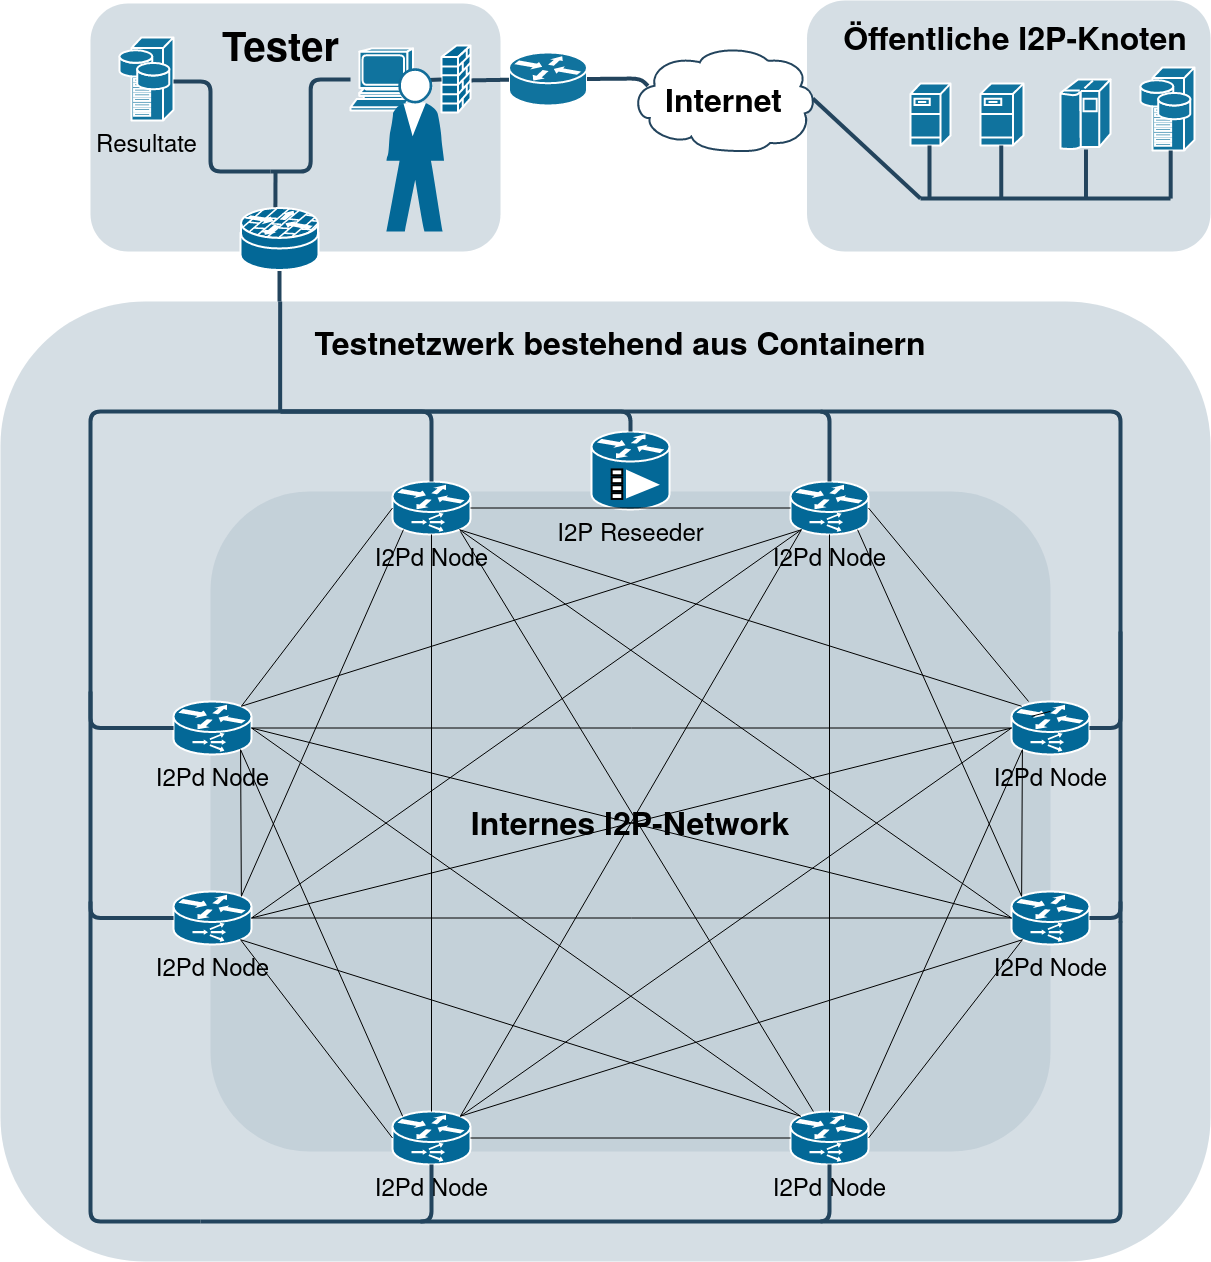
\includegraphics[width=1.0\textwidth]{i2p-testnetwork.png}
  \caption{I2P Testnetwork}\label{fig:i2p-testnetwork}
\end{figure*}

Bei der Firewall handelt es sich entweder um das Hostsystem (VM-Network) für das Testnetzwerk selber, welche die I2P-Knoten hostet, oder um einen extra Container der aller outgoing traffic kontrolliert.
Wichtig ist das der Tester, welcher das Netzwerk erstellt und die Tests durchführt sich auch ausserhalb des Testnetzwerkes befindet, um ungewollte Einflüsse zu vermeiden.

Die I2P-Knoten sind als Router dargestellt und befinden sich eigentlich alle in zwei Netzwerken gleichzeitig. Das normale IP Netzwerk und das I2P-Netzwerk.
Am Ende des Tests müssen die Testresultate an einem sicheren Ort ausserhalb des Testnetzwerks abgelegt werden, damit diese später analysiert werden können (Result). (ResultDB)

In der \lstinline|i2pd| Konfiguration gibt es zusätzlich das \lstinline|familiy| tag, welches die Knoten als zusammenhängend markieren würde, würden diese aus Versehen mit dem echten I2P Netzwerk reden. Dies ist auch interessant bezüglich Tests die am echten Netzwerk durchgeführt werden sollen.

%TODO: fullmesh?

\section{Bootstrapping und Verbindungsgrad der Knoten}

% TODO: in 3.2.1 Nötig weil isoliert
Ganz zu Beginn, wenn ein Knoten dem I2P Netzwerk beitritt muss dieser Wissen wo mindestens ein anderer Knoten ist.
Um die erste Liste von Knoten zu erhalten damit Knoten dem Netzwerk beitreten können, muss die liste von Knoten im Netzwerk zu beginn des Tests ''geseedet'' mit einer liste von Bekannten Knoten.
Es wird also entweder ein Floodfill-Router benötigt oder ein separater Reseed-Server.

Ohne einen Reseed server ist dies möglich mit einem floodfill reseed:

\url{https://i2pd.readthedocs.io/en/latest/tutorials/floodfill-bootstrap/}

Dies würde es auch erlauben ein Testnetzwerk zu erstellen, deren Knoten nicht von allen anderen Knoten Bescheid wissen.


Um bessere empirische Aussagen machen zu können, sollte das Testnetzwerk so gut wie möglich das öffentliche I2P-Netzwerk abbilden \seereq{EVAL}.


\section{Messen der Ressourcenauslastung}\label{sec:ressourcenauslastung}

%TODO: in kapitel latenz

Die Messung der Ressourcenauslastung der Knoten könnte sinnvoll sein aus mehreren Gründen.
Gerät ein Knoten oder die Hostsysteme für das Testnetzwerk in Ressourcenengpässe beeinflusst dies auch die Resultate.
Dies ist insbesondere wichtig enorm wichtig bei Latenzmessungen, denn diese werden somit fehlerhaft und nicht reproduzierbar \seereq{TREP}.

\begin{itemize}
    \item Somit kann sichergestellt werden, dass das Testnetzwerk nicht so gross skaliert wurde, bzw. wie weit es skaliert werden kann \seereq{TSCL}.
    \item Um sicherzustellen, dass ein Flaschenhals im Netzwerk nicht durch zu wenig Ressourcen verursacht sind \seereq{TPER}.
    \item Äussere einflüsse wie Ressource-Exhaustion vermeiden, dies verbessert auch die Reproduzierbarkeit \seereq{TREP}.
    \item Messung der Test-Performance
\end{itemize}

Gemessen werden sollte:

\begin{itemize}
    \item Netzwerkbandbreite (kbits/sec)
    \item CPU gebrauch (in Prozent)
    \item RAM Verwendung (in Prozent)
    \item Disk I/O (read/write, kbits/sec)
    \item Freier Speicherplatz
\end{itemize}

Es wird erwartet, dass der Workload von I2P vor allem Netzwerklastig (weiterleiten über mehrere Knoten) und Prozessorlastig (Verschlüsselung) ist.
Da es sich hier um ein virtuelles Container-Netzwerk handelt, heisst dass die Last auf dem Netzwerk sich auch in der Prozessorlast zeigen wird.
Zudem wird nicht wenig Arbeitsspeicher verwendet, um die benötigte Anzahl Container und Knoten zu betreiben.
